
\pdfminorversion=4
\documentclass[xcolor=dvipsnames]{beamer}
\usepackage{tabls}
\usepackage{graphicx}
%\usepackage{animate}
\usepackage{xcolor}

%tikz stuff
\usepackage{tikz}
\usetikzlibrary{shapes.geometric, arrows}
\tikzstyle{startstop} = [rectangle, rounded corners, minimum width=2cm, text
    width=1.8cm, minimum height=1cm,text centered, text=white,draw=black, fill=Gray!140]
\tikzstyle{io} = [trapezium, trapezium left angle=70, trapezium right angle=110,
minimum width=0.5cm, minimum height=1cm, text centered, draw=black,
fill=blue!20!Gray!90!,text=white]
\tikzstyle{process} = [rectangle, minimum width=2cm, minimum height=1cm, text
centered, text width=2cm, draw=black, text=white,fill=Gray!140!blue!70!white]
\tikzstyle{decision} = [diamond, minimum width=3cm, minimum height=1cm, text
centered, draw=black, fill=Gray!,text=white]
\tikzstyle{arrow} = [thick,line width=0.6mm,->,>=stealth]
\tikzstyle{arrow1} = [dashed,->,>=stealth]
\setbeamertemplate{navigation symbols}{}
\setbeamertemplate{footline}[frame number]

%\definecolor{myblue}{rgb}{0.7, 0.7, 60.0}
\definecolor{mylightblue}{rgb}{1,1,1}
\newcommand*{\boxedcolor}{blue}
\makeatletter
\renewcommand{\boxed}[1]{\textcolor{\boxedcolor}{%
  \fbox{\normalcolor\m@th$\displaystyle#1$}}}
\makeatother
\usepackage{hyperref}

\newcommand{\backupbegin}{
   \newcounter{framenumberappendix}
   \setcounter{framenumberappendix}{\value{framenumber}}
}
\newcommand{\backupend}{
   \addtocounter{framenumberappendix}{-\value{framenumber}}
   \addtocounter{framenumber}{\value{framenumberappendix}} 
}
\renewcommand{\u}[1]{\underline{#1}}

\newcommand{\iso}[2]{${}^{{#2}}${#1} }
\newcommand{\nubar}[0]{$\overline{\nu}$ }
\newcommand{\keff}[0]{\ensuremath{{k}_{\textsf{eff}}} }
\newcommand{\expect}[1]{E[#1] }
\newcommand{\colg}[1]{{\color{ForestGreen} #1}}
\newcommand{\coly}[1]{{\color{yellow} #1}}
\newcommand{\colb}[1]{{\color{blue} #1}}
\newcommand{\colr}[1]{{\color{red} #1}}
\usepackage{amsfonts}
\newlength{\wideitemsep}
\setlength{\wideitemsep}{8pt}
%\addtolength{\wideitemsep}{5pt}
\let\olditem\item
\renewcommand{\item}{\setlength{\itemsep}{\wideitemsep}\olditem}

\newcommand{\N}{\mathbb{N}}
\newcommand{\Z}{\mathbb{Z}}
\newcommand{\deriv}[2]{\frac{\mathrm{d} #1}{\mathrm{d} #2}}
\newcommand{\pderiv}[2]{\frac{\partial #1}{\partial #2}}
\newcommand{\bx}{\mathbf{X}}
\newcommand{\ba}{\mathbf{A}}
\newcommand{\by}{\mathbf{Y}}
\newcommand{\bj}{\mathbf{J}}
\newcommand{\bs}{\mathbf{s}}
\newcommand{\B}[1]{\ensuremath{\mathbf{#1}}}
\newcommand{\Dt}{\Delta t}
\renewcommand{\d}{\mathsf{d}}
\newcommand{\mom}[1]{\langle #1 \rangle}
\newcommand{\xl}{{x_{i-1/2}}}
\newcommand{\xr}{{x_{i+1/2}}}
\newcommand{\il}{{i-1/2}}
\newcommand{\ir}{{i+1/2}}

\AtBeginSection[]
{
    \begin{frame}<beamer>
        \frametitle{Outline}
        \tableofcontents[currentsection]
    \end{frame}
}

\setbeamerfont{frametitle}{size=\normalsize}
\setbeamerfont{normal font}{size=\tiny}

\graphicspath{{figures/}}

\usepackage{verbatim}
\usepackage{comment}
\usepackage[]{datetime}
\usepackage{multirow}

\newcommand{\thedate}{\today}


\setlength{\tabcolsep}{1.05cm}

%Aggie-themed
\pgfdeclareimage[height=0.1in]{TAMUlogo}{tamu_engineering.png}
\logo{\raisebox{-8pt}{\pgfuseimage{TAMUlogo}}}
\titlegraphic{\centering\begin{tabular}{c}

\includegraphics[height=0.18\textheight]{tamu_seal.png}\end{tabular}}
%Michigan-themed
%\pgfdeclareimage[height=0.1in]{UMlogo}{michigan_engineering.png}
%\logo{\raisebox{-8pt}{\pgfuseimage{UMlogo}}}
%\titlegraphic{
\includegraphics[height=0.2\textheight]{michigan_block_m.png}}


%%%%%%%%%%%%%%%%%%%%%%%%%%%%%%%%%%%%%%%%%%%%%%%%%%%%%%%%%%%%%%%
% Optional packages, used to show off certain tricks

\newlength \figwidth
\setlength \figwidth {0.5\textwidth}

\setlength{\leftmargin}{-2cm}
\setlength{\rightmargin}{-2cm}

%%%%%%%%%%%%%%%%%%%%%%%%%%%%%%%%%%%%%%%%%%%%%%%%%%%%%%%%%%%%%%%

\usepackage[english]{babel}
\usetheme{Frankfurt}

%Make it Aggie Maroon
\usecolortheme[RGB={80,0,0}]{structure}  
%Or Michigan Blue
%\usecolortheme[RGB={0,0,153}]{structure}  
%Or Michigan Maize
%\usecolortheme[RGB={255,204,0}]{structure}  

  % This will typeset only the frames (or slides) that have the given label ("current" in this case).

\title{Second-Order Discretization in Space and Time for Grey S$_2$-Radiation Hydrodynamics}
    \author{{\large Simon R. Bolding, Joshua E. Hansel, \& Jim E. Morel}}
\date{16 October 2015 \\ \vspace{0.05in} {CLASS seminar}}
\subject{}
%\institute{Los Alamos National Laboratory}

% \classificationlevel{SECRET/RD}
% \transmissible{}

%\reportnum{\textcolor{blue}{SAMPLE TEMPLATE ONLY \\ Contains NO Classified
%Information}}

%\dissableframenumber
\begin{document}

\begin{frame}
    \titlepage \vspace{-0.213in}
    \begin{center}
    \end{center}    
\end{frame}

\setlength{\tabcolsep}{6pt}

\begin{frame}
\frametitle{Outline}
\begin{minipage}{0.061\linewidth}
\hfill                      
\end{minipage}
\begin{minipage}{0.8\linewidth}
\tableofcontents[
hideothersubsections,
sectionstyle=show,
subsectionstyle=hide
]
\end{minipage}

\end{frame}


\section{Overview}
\subsection{}

\begin{frame}
    \frametitle{What is radiation hydrodynamics?}
    \begin{itemize}
        \item Thermal radiative transfer coupled to material motion
            \begin{itemize}
                \item Useful for inertial confinement fusion and astrophysics calculations
            \end{itemize}
    \end{itemize}
        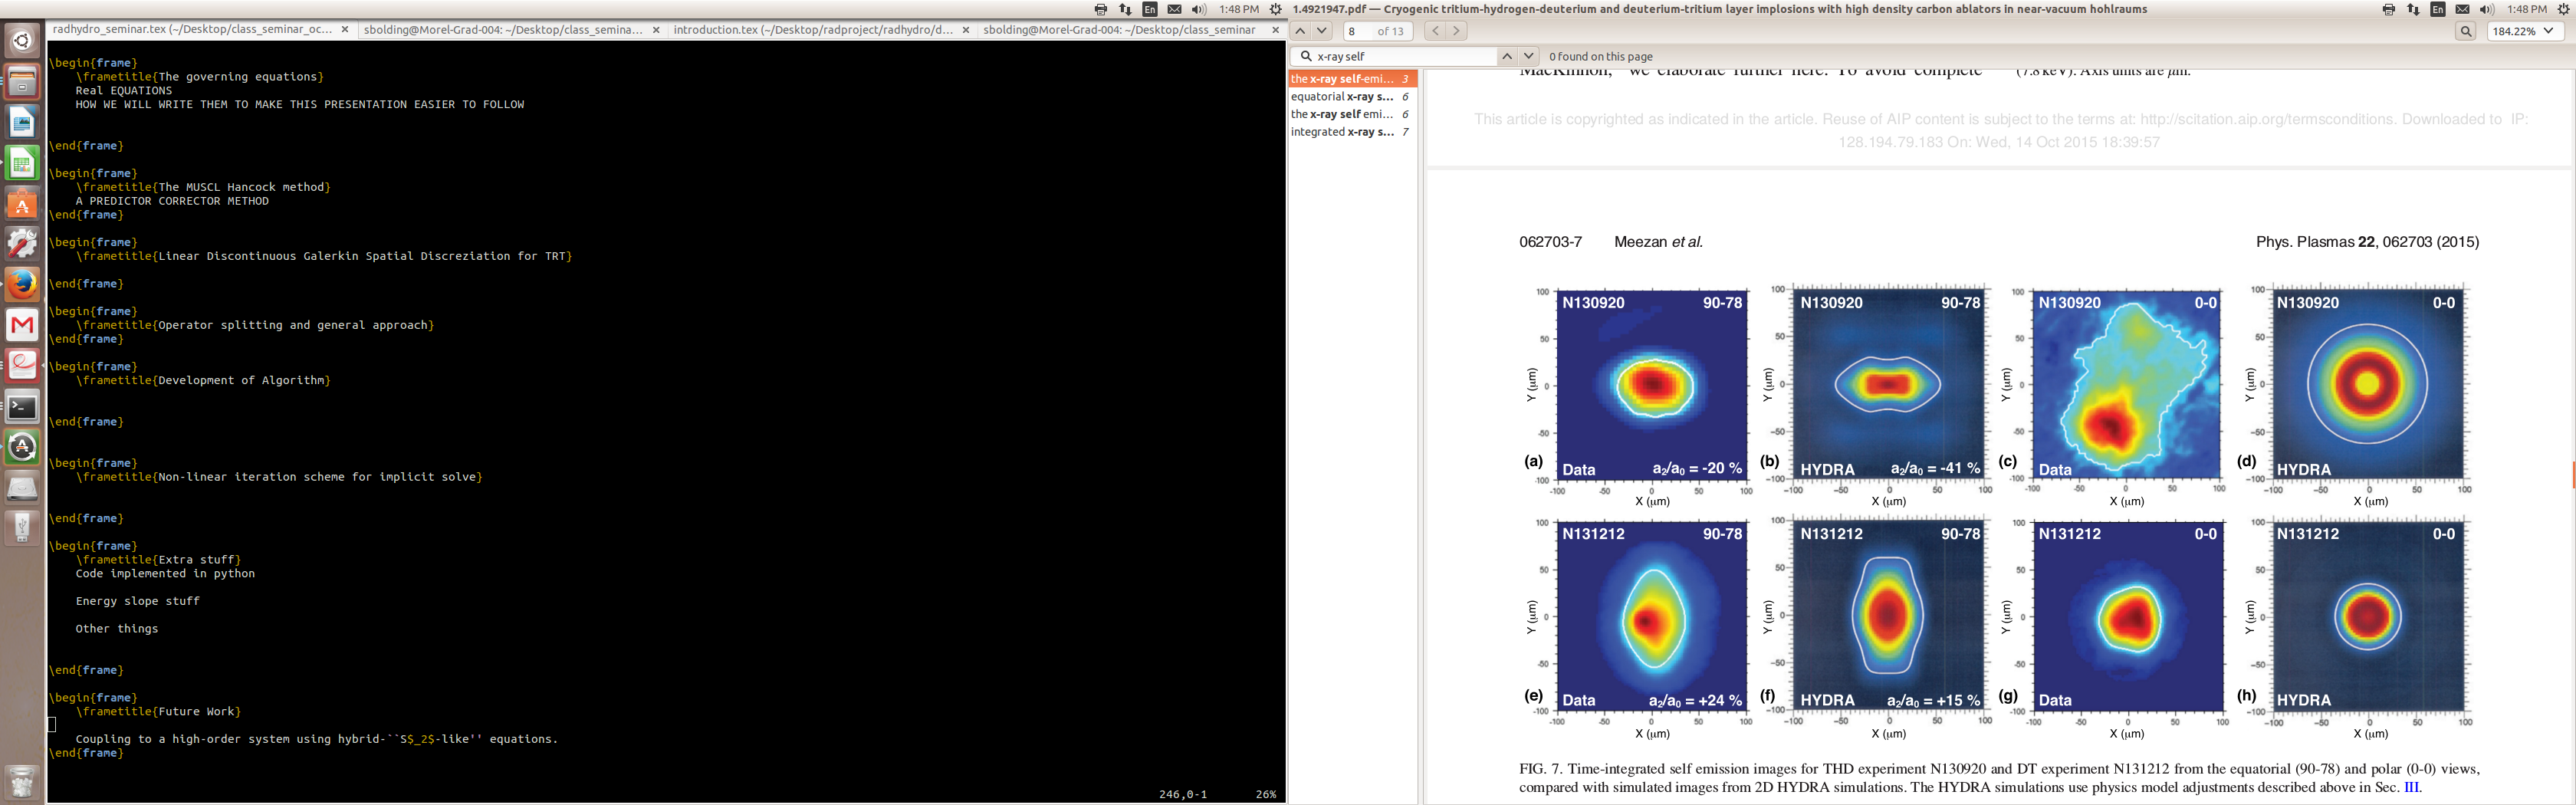
\includegraphics[width=0.5\textwidth,trim=28in 2in 6in 5in,clip]{nif.png}
\end{frame}

\begin{frame}
    \frametitle{Example of a 1D Radiative Shock Solution}
    \begin{block}{Goal of this project}
        \begin{itemize}
            \item
     Extended work by Edwards and Morel for a method that is second-order in
     \colb{space} and \colb{time}
 \item We applied to S$_2$ equations which allows for conservation of momentum 
     \end{itemize}
 \end{block}
\end{frame}

\begin{frame}
    \frametitle{The governing equations}

    
\end{frame}


\begin{frame}
    \frametitle{The MUSCL Hancock method}
    A PREDICTOR CORRECTOR METHOD
\end{frame}

\begin{frame}
    \frametitle{Linear Discontinuous Galerkin Spatial Discreziation for TRT}

\end{frame}

\begin{frame}
    \frametitle{Operator splitting and general approach}
\end{frame}

\begin{frame}
    \frametitle{Development of Algorithm}


\end{frame}


\begin{frame}
    \frametitle{Non-linear iteration scheme for implicit solve} 


\end{frame}

\begin{frame}
    \frametitle{Extra stuff}
    Code implemented in python

    Energy slope stuff

    Other things


\end{frame}

\begin{frame}
    \frametitle{Future Work}

    Coupling to a high-order system using hybrid-``S$_2$-like'' equations.
\end{frame}


\begin{frame}
    \frametitle{A High-Order Low-Order Solution to a Transport Problem}
        \begin{itemize}
            \item[]<1-> \begin{block}{Basic Idea} Build a low-order (LO) system that can be efficiently solved,
                such that it preserves a high-order (HO) solution from MC simulations \end{block}
                \vspace{-0.3in}
              \item<3-> \textbf{LO system} is lower-dimensional,  ``S$_2$-like" equations
                \begin{itemize}
                    \item<3-> Handles scattering and fission source iterations
                    \item<3-> Useful for coupled physics and non-linear systems
                    \item<3-> Produces \colb{FE representation of sources} for HO system
                  %  \item Consistency terms derived directly from transport equation
                \end{itemize}
            \item<4-> \textbf{HO system} is a fixed-source, pure absorber transport problem
                \begin{itemize}
                    \item  MC does not directly determine $\keff$ or fission source,
                        only used to \colb{evaluate consistency terms} 
                    \item We will solve the HO system with ECMC
                \end{itemize}
        \end{itemize}
\end{frame}

\begin{frame}
    \frametitle{Overview of Exponentially Convergent Monte Carlo}
    \begin{itemize}
        \item Iterative form of Residual Monte Carlo
      \begin{itemize}
          \item Each batch tallies the \colb{error} in current estimate of solution, which
            is a transport problem with a reduced source
    \item Can reduce statistical error \colb{globally} $\propto e^{-\alpha N}$
\end{itemize}
            \begin{itemize}
                \item Does not make difficult problems easier 
            \end{itemize}\pause
        \item Requires a \colr{discretized} form of the angular flux            \begin{itemize}
                \item Use \colb{projection} onto space-angle FE mesh
        \item Adaptive mesh refinement mitigates truncation error, allowing convergence to be maintained
    \end{itemize}
    \end{itemize}
\end{frame}



\begin{frame}
    \frametitle{High-Order Low-Order Algorithm}
    \fontsize{10}{11.0}\selectfont
    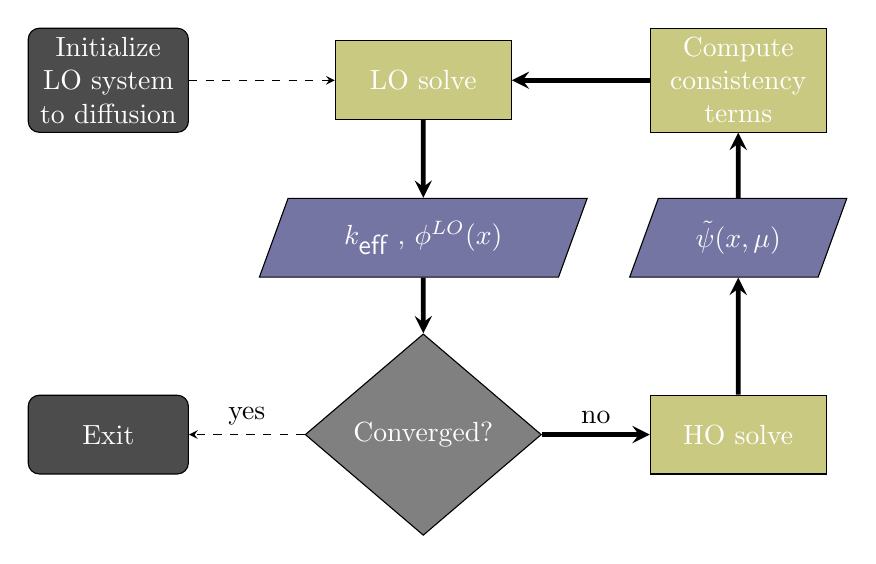
\begin{tikzpicture}[node distance=2cm]
        \node (start) [startstop] {Initialize LO system to diffusion};
        \node (in1) [process, right of=start, xshift=2cm] {LO solve};
        \node (pro1) [io, below of=in1] {\keff, $\phi^{LO}(x)$};
        \node (dec1) [decision, below of=pro1, yshift=-0.5cm] {Converged?};
        \node (pro2a) [startstop, left of=dec1, xshift=-2.0cm] {Exit};
        \node (pro2b) [process, right of=dec1, xshift=2cm] {HO solve};
        \node (out1) [io, above of =pro2b, yshift=0.5cm] {$\tilde{\psi}(x,\mu)$};
        \node (cons) [process, above of=out1] {Compute consistency terms};
        \draw [arrow1] (start) -- (in1);
        \draw [arrow] (in1) -- (pro1);
        \draw [arrow] (pro1) -- (dec1);
        \draw [arrow] (dec1) -- node[anchor=south] {no} (pro2b);
        \draw [arrow1] (dec1.west) -- node[anchor=south] {yes} (pro2a);
        \draw [arrow] (pro2b) -- (out1);
        \draw [arrow] (cons) -- (in1);
        \draw [arrow] (out1) -- (cons);
    \end{tikzpicture}
\end{frame}




\section{Low-Order Solver}
\subsection{}

\begin{frame}
    \frametitle{LO Discretization \& Space-Angle Moments}
    \begin{itemize}
        \item Linear discontinuous (LD) FE in space and half range
            angular averages 
    \end{itemize}
    \begin{centering}
    \begin{tikzpicture}
    \node[anchor=south west,inner sep=0] at (0,0) {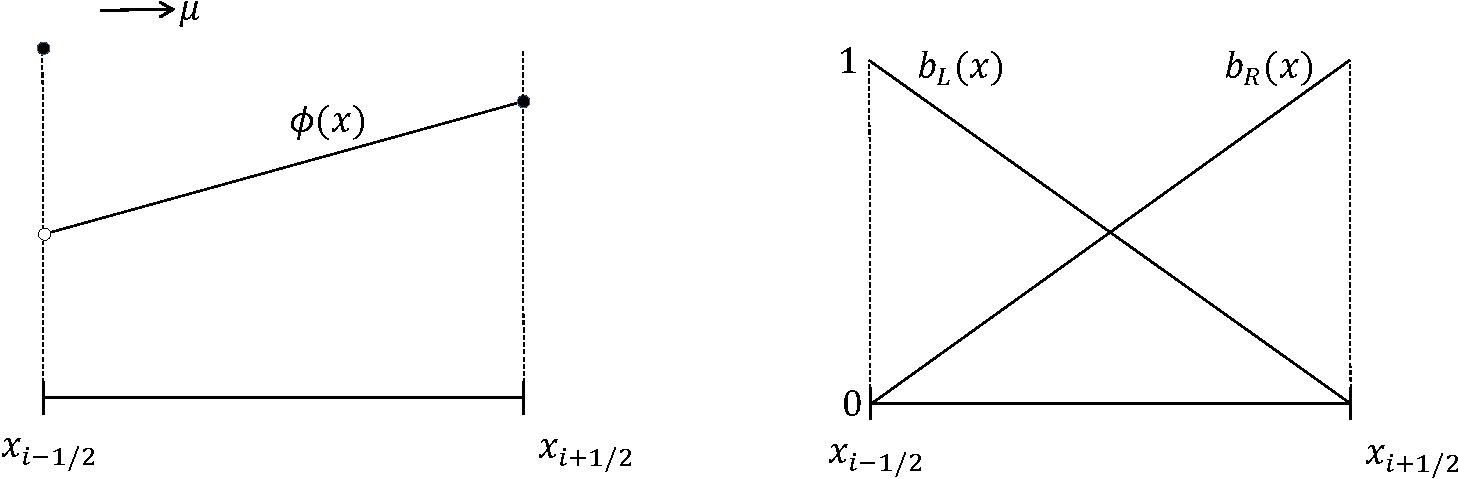
\includegraphics[width=0.9\textwidth]{LD.pdf}};
    \node at (2.109,2.50853) {\scriptsize ${^+}$};
\end{tikzpicture}
    \end{centering}
    \begin{itemize}
    \pause
\item \emph{Examples} of moments:
    \end{itemize}
    \begin{center}
    \begin{tabular}{cc}
        \underline{Spatial: left basis} & \underline{Angular: positive flow} \\ 
        $ {\displaystyle \mom{\cdot}_{L,i} = \frac{2}{h_i} \int_{x_\il}^{x_\ir}
        b_{L,i}(x)(\cdot) \d x \quad }$  & ${ \quad \displaystyle \phi^+(x) = 2\pi\int_0^1 \psi(x,\mu) \d \mu}$
    \end{tabular}
    \end{center}

\end{frame}




\begin{frame}
    \frametitle{Forming LO Equations Over an Element}
    \begin{itemize}
        \item Taking moments of TE yields \colb{4 equations}, per cell $i$, e.g.
        {\small
        \begin{multline*}\label{lo_tran}
    -2{\mu}_{i-1/2}^{+} \phi_{i-1/2}^{+} + \mom {\mu}_{L,i}^{+}
  \mom{\phi}_{L,i}^{+}
  +  \mom\mu_{R,i}^{+}
  \mom{\phi}_{R,i}^{+} + \Sigma_t h_i \mom{\phi}_{L,i}^+ \\-  \frac{\Sigma_s h_i}{4\pi} \left( \mom{\phi}_{L,i}^{+} +
  \mom\phi_{L,i}^{-}\right) = \frac{1}{\keff} \frac{\nu \Sigma_fh_i}{4\pi}\left( \mom{\phi}_{L,i}^{+} +
  \mom\phi_{L,i}^{-}\right)
\end{multline*}}
        \item Cell unknowns are \colb{moments}: $\mom{\phi}_{L,i}^{+}$, $\mom{\phi}_{R,i}^{+}$,
        $\mom{\phi}_{L,i}^{-}$, $\mom{\phi}_{R,i}^{-}$ 

    \item \pause To close system, need angular consistency terms  and spatial
        closure
    \begin{itemize} 
        \item Estimate \emph{average $\mu$} terms from HO solution
        \item Use the LD spatial closure, consistent with our HO solver
    \end{itemize}
    \end{itemize}

\end{frame}


\begin{frame}
    \frametitle{Computing LO Consistency terms from HO Solution}
    \begin{itemize}
        \item For $\mu>0$, $L$ moment
            \begin{equation*}\label{consistency}
\mom{{\mu}}_{L,i}^{+} \simeq \frac{\displaystyle 
 \int\limits_0^1 \int\limits_\xl^\xr \mu \, b_{L,i}(x) \tilde \psi^{HO}(x,\mu) \d x \d \mu } 
{\displaystyle \int\limits_0^1 \int\limits_\xl^\xr \, b_{L,i}(x)
\tilde \psi^{HO}(x,\mu) \d x \d \mu } 
    \end{equation*}
\item \pause ECMC gives LDFE representation of $\tilde  \psi^{HO}(x,\mu)$
    \begin{itemize} 
        \item Evaluate consistency terms directly
        \item For initial solve, use S$_2$: $\mom{\mu}^\pm = \pm \frac{1}{\sqrt{3}}$ 
    \end{itemize}
    \end{itemize}
\end{frame}

\begin{frame}
    \frametitle{Solving LO System with Power Iteration}
    \begin{itemize}
        \item Global System: \hspace{0.8in}${\displaystyle \B D(\mu^{HO}) \Phi = \frac{1}{\keff} \B F \Phi}$
     \end{itemize}
     \pause
     \begin{block}{Algorithm}
         \begin{enumerate}
        \item Guess $\Phi^{(0)}$ and $\keff^{(0)}$
        \begin{align*}
    \Phi^{(l+1)} = \frac{1}{\keff^{(l)}} \B D^{-1} \B F \Phi^{(l)} \\
    \quad \keff^{(l+1)} = \keff^{(l)}\frac{ \int \nu \Sigma_f \phi^{(l+1)} \d
    x}{ \int \nu \Sigma_f \phi^{(l)}\d x }.
        \end{align*} \pause
    \item \colb{Accelerate} $\Phi^{(l+1)}$ and $\keff^{(l+1)}$ after each power iteration
        with Nonlinear Krylov Acceleration (NKA)
    \item Converge $\Delta \Phi^{(l)}$ and $\Delta \keff^{(l)}$ 
     \end{enumerate}
    \end{block}
\end{frame}

\section{High-Order Solver}
\subsection{}


\begin{frame}
    \frametitle{Space-Angle LDFE Mesh}
    \noindent
    \fontsize{9.89}{5.0}\selectfont
    \begin{minipage}[t]{0.36\linewidth}
        \centering
        \scalebox{0.8}{
        \begin{tikzpicture}
            \draw (1,1) rectangle (4,4);
            \node[draw,circle,inner sep=1.2 pt,fill] at (2.5,2.5) {};
            \node[above] at (2.5,2.5) {$(x_i,\mu_j)$};
            \draw (1.0,0.4) -- (1.0,0.6) node[below, pos=0.4] {$x_{i-1/2}$};
            \draw (4.0,0.4) -- (4.0,0.6) node[below, pos=0.4] {$x_{i+1/2}$};
            \draw (0.4,1.0) -- (0.6,1.0) node[left, pos=0.4] {$\mu_{j-1/2}$};
            \draw (0.4,4.0) -- (0.6,4.0) node[left, pos=0.4] {$\mu_{j+1/2}$};
            \draw [thick,->] (0.5,0.5) -- (5,0.5) node[anchor=north west] {$x$};
            \draw [thick,->] (0.5,0.5) -- (0.5,5) node[anchor=east] {$\mu$};
        \end{tikzpicture}
    }
    \end{minipage}%
    \begin{minipage}[t]{0.70\linewidth}
        \vspace{-1.6in}
        \hspace{0.5in}
        \begin{itemize}
            \item {\small $\displaystyle \tilde \psi(x,\mu)$} is linear over each
                cell, \colb{preserving} $0^{\text{th}}$ and $1^{\text{st}}$ moment in $x$
                and $\mu$
            \item Use path-length estimators of flux to approximate moments e.g.
            {\small
            \begin{align*}
                \mom{\psi}_{\mu,ij} &= \frac{6}{h_{\mu}^2h_x}
             \iint\limits_\mathcal{D} (\mu-\mu_i) \psi(x,\mu) \d x \d \mu 
        \end{align*}}    
        \end{itemize}
    \end{minipage}
    \pause
    \begin{itemize}
       \item Use standard LD and upwinding to get face terms
    \end{itemize}
\end{frame}



\begin{frame}
    \frametitle{High Order System and ECMC Algorithm}
    \begin{itemize}
        \item \colb{Pure absorber} transport problem
        \begin{align*}
            \left[\mu \pderiv{}{x} + \Sigma_t\right]\psi(x,\mu)
            &= \boxed{\frac{1}{4\pi}\left(\Sigma_s + \frac{\nu
    \Sigma_f}{\keff^{\colb{LO}}}\right)
        {\phi^{\colb{LO}}(x)}} \\ 
         \B L \psi &= q^{LO}
     \end{align*}
        \vspace{-0.3in}
        \end{itemize}\pause
        \begin{block}{ECMC Algorithm}
         \begin{itemize}
             \item Residual Equation: \vspace{-0.33in}
                 \begin{align*} 
                     \hspace{0.5in}\displaystyle \B L (\psi - \tilde\psi^{(m)}) &=  q^{LO} - \B L \tilde\psi^{(m)} \\
                     \B L \tilde\epsilon^{(m)} &= \tilde r ^{(m)} 
        \end{align*}
            \vspace{-0.3451in} \pause
        \item Compute $\tilde{\epsilon}^{(m)} = \B L^{-1} \tilde{r}^{(m)}$ with MC,
            \colb{projecting} the solution  
        \item Update: $\tilde\psi^{(m+1)} = \tilde\psi^{(m)} + \tilde \epsilon^{(m)}$
        \begin{itemize}
            \item \pause If $\tilde{\epsilon}$ is reduced each batch, \colb{exponential convergence
                achieved}
            \item $h$-refine when $\epsilon(x,\mu)$ not represented sufficiently
        \end{itemize}
    \item Repeat until $\| \tilde \epsilon \|_2 < \textsf{tol}\times \| \psi \|_2$
    \end{itemize}
\end{block}

\end{frame}


\begin{frame}
    \frametitle{Other MC Details}
  \begin{block}{Improving Statistics and Efficiency}
    \begin{itemize}
        \item Particles \colb{only stream:} $w(s)=w_0 e^{-\Sigma_t s}$
            \pause
        \item Cell-wise, global representation accommodates \colb{stratified} sampling
        \begin{itemize}
            \item $N_{ij} \propto{|r_{ij}(x,\mu)|}$
            \item Force $N_{ij} \geq N_{\min}$ 
        \end{itemize}
\item \pause Initialize $\tilde{\psi}(x,\mu)$ to latest HO solution for first batch
\end{itemize}
    \end{block}

\end{frame}
\section{HOLO Algorithm}
\subsection{}

\begin{frame}
    \frametitle{High-Order Low-Order Algorithm}
    \fontsize{10}{11.0}\selectfont
    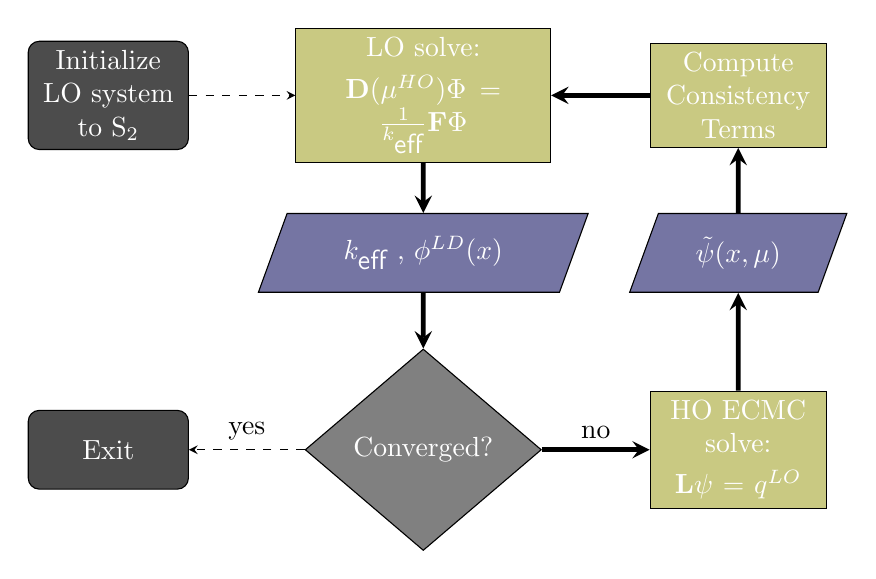
\begin{tikzpicture}[node distance=2cm]
        \node (start) [startstop] {Initialize LO system to S$_2$};
        \node (in1) [process, right of=start, xshift=2cm, text width=3cm] {LO solve:\vspace{0.041in}
        $\B D(\mu^{HO})\Phi = \frac{1}{\keff}\B F\Phi$};
        \node (pro1) [io, below of=in1] {\keff, $\phi^{LD}(x)$};
        \node (dec1) [decision, below of=pro1, yshift=-0.5cm] {Converged?};
        \node (pro2a) [startstop, left of=dec1, xshift=-2.0cm] {Exit};
        \node (pro2b) [process, right of=dec1, xshift=2cm] {HO ECMC solve:\vspace{0.041in} $\B L \psi =
        q^{LO}$};
        \node (out1) [io, above of =pro2b, yshift=0.5cm] {$\tilde{\psi}(x,\mu)$};
        \node (cons) [process, above of=out1] {Compute Consistency Terms};
        \draw [arrow1] (start) -- (in1);
        \draw [arrow] (in1) -- (pro1);
        \draw [arrow] (pro1) -- (dec1);
        \draw [arrow] (dec1) -- node[anchor=south] {no} (pro2b);
        \draw [arrow1] (dec1.west) -- node[anchor=south] {yes} (pro2a);
        \draw [arrow] (pro2b) -- (out1);
        \draw [arrow] (cons) -- (in1);
        \draw [arrow] (out1) -- (cons);
    \end{tikzpicture}
\end{frame}




\section{Test Problems}
\subsection{}
\begin{frame}
    \frametitle{\coly{Critical slab benchmark}}
    \fontsize{9}{5.0}\selectfont
    \begin{block}{Problem Parameters}
    \begin{itemize}
        \item $k_\infty = 2.29$, $\Sigma_t = 0.326$ cm$^{-1}$
        \item Initially 100 $x$ \& 20 $\mu$ cells
        \item Adaptive HO convergence
    \end{itemize}
    \pause
    \end{block}
    \begin{minipage}{0.49\textwidth}
    \begin{figure}
    \centering
    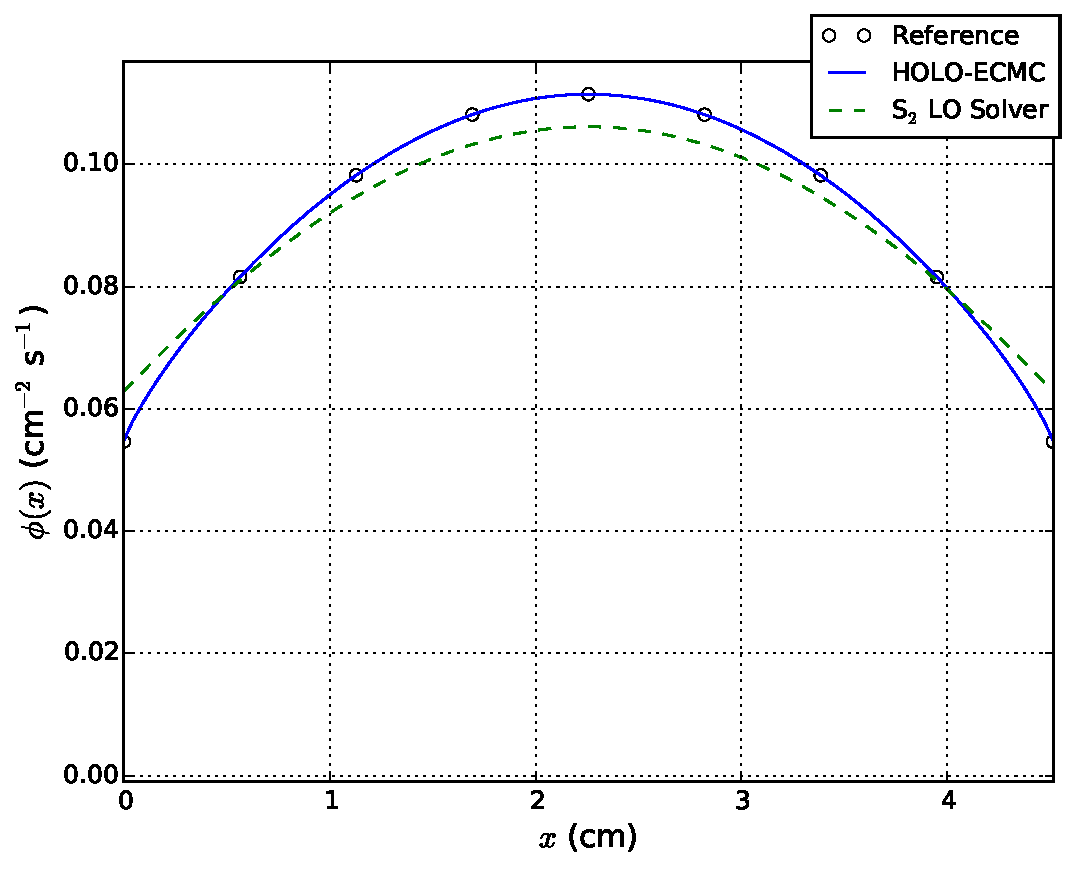
\includegraphics[width=1.09\textwidth]{sood_fiss_src.pdf}
    \end{figure}
    \end{minipage}
    \begin{minipage}{0.49\textwidth}
    \begin{itemize}
        \item $|\Delta \Phi|_{\text{rel}} < 10^{-4}$ in 4 outer iterations, using            $\sim2.4\times10^7$ histories
        \item For 10 independent simulations:{\large
        	\begin{center}
            \begin{tabular}{|cc|} \hline
                  $\overline{\keff}$ & $0.999998$ \\ 
                    $\sigma(\keff)$ & 0.4 pcm \\
                   $\Delta k_{\text{eff}}^{\max}$  & $1.1$ pcm \\
                $\overline{\sigma_{\text{rel}}(\phi_i)}$ & 1.4 pcm\\ \hline
           \end{tabular}
           \end{center}}
    \end{itemize}
    \end{minipage}
\end{frame}

\begin{frame}
    \frametitle{\coly{Optically thick, near-critical slab}}
    \fontsize{9}{5.0}\selectfont
    \begin{block}{Problem Parameters}
    \begin{itemize}
        \item $k_\infty = 1$, $\Sigma_t = 5.0$ cm$^{-1}$, $\Sigma_s=4.5$ cm$^{-1}$,
            DR$\simeq$\textbf{0.984}
        \item Relative Tolerance of 1.0E-05 for HO and LO solvers, 1.0E-04 outer 
    \end{itemize}\pause
    \end{block}
    \begin{minipage}{0.49\textwidth}
    \begin{figure}
    \centering
    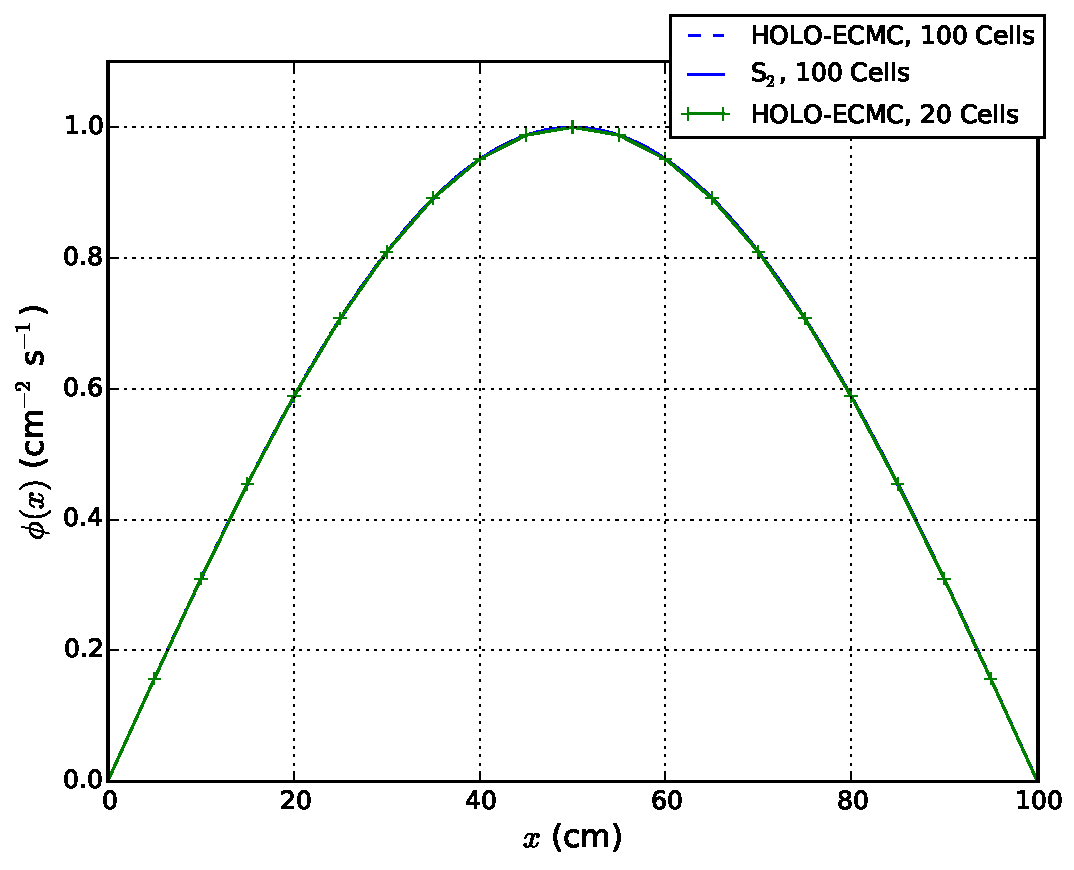
\includegraphics[width=1.08\textwidth]{highdr_fiss_src.pdf}
    \end{figure}
    \end{minipage}
    \begin{minipage}{0.49\textwidth}
        \begin{itemize}
            \item LO fission source convergence:
            \begin{itemize}
                \item \hspace{-0.1in} PI: \textbf{389} iterations
                \item \hspace{-0.1in} NKA: \textbf{27} iterations
            \end{itemize}
        \item 3 outer iterations, 4.4$\times 10^6$ total histories
            \item $\keff = 0.99793$ 
        \end{itemize}
    \end{minipage}
\end{frame}

\begin{frame}
    \fontsize{9}{5.0}\selectfont
    \frametitle{Comparison of statistical noise for standard and ECMC HO solvers}
    \begin{block}{}
        One HOLO solve, with a fixed $1.5\times10^5$ histories. Comparison of
            \colr{ECMC} with 5 batches and standard MC (\colb{SMC}) 
    \end{block}\pause
  \begin{figure}
    \centering
    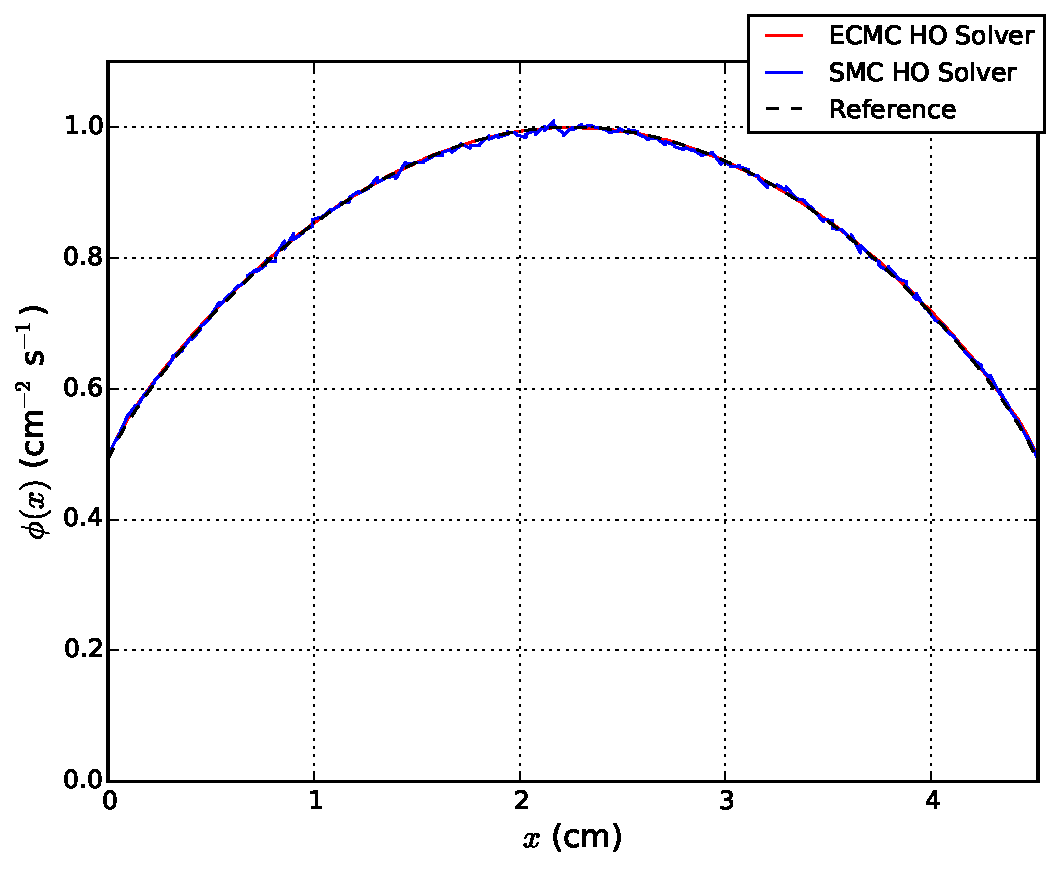
\includegraphics[width=0.589\textwidth]{sood_smc_compare.pdf} 
  \end{figure}
  \pause
  \begin{equation*}
  \boxed{
  \displaystyle\frac{\|\sigma(\psi^{SMC})\|}{\|\tilde\epsilon^{ECMC}\|
  +\|\sigma(\epsilon^{ECMC})\| }=16}
  \end{equation*}

\end{frame}

\section{Conclusions}
\subsection{}

\begin{frame}
    \frametitle{Observations \& Future Work}
    \begin{itemize}
        \item Able to solve for $\keff$ and fission source with HOLO method
        \begin{itemize}
            \item Pure absorber histories are more efficient than standard MC simulations
            \item ECMC works well in HOLO context
        \end{itemize}
        \pause
        \item Stratified source sampling produces less variance than a constant
            number of histories per cell \pause
        \item Need to use the estimated statistical error in tallies for $\tilde\epsilon(x,\mu)$ 
        \begin{itemize}
            \item Run more particles on refined meshes, monitoring local error
            \item Source biasing \pause
         \end{itemize}
     \item Working on application to \colb{thermal radiative transfer} problems
    \end{itemize}

\end{frame}

\begin{frame}
    \frametitle{Marshak Wave Problem, Radiation Temperature Profile}
  \centering
  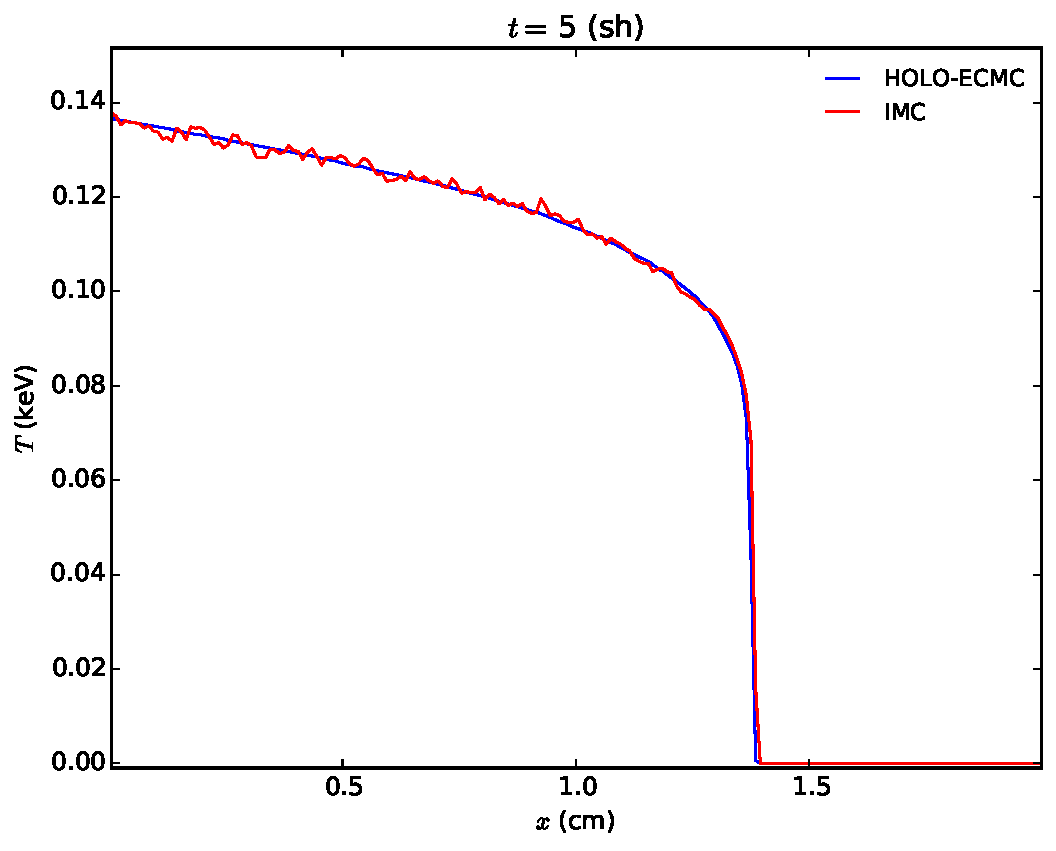
\includegraphics[width=0.69\linewidth]{marshak_200_compare.pdf}
  \begin{itemize}
      \item \colr{IMC}: 100,000 particles per time step
      \item \colb{HOLO-ECMC}: 15,000 particles per time step
  \end{itemize}

\end{frame}

\date{21 November 2014}

\begin{frame}
    \frametitle{{\LARGE\coly{Questions?}}}
    \titlepage \vspace{-0.113in}
\end{frame}

\backupbegin
\appendix

\title{Backup Slides}
\author{}
\date{}





\begin{frame}
    \frametitle{ECMC procedure}
    {
    \begin{block}{Algorithm}
    \begin{enumerate}
        \item $\tilde \psi^{(0)}=\tilde \psi$ or from last batch this time step
        \item Using Monte Carlo, $\epsilon^{(m)} = \B L^{-1} \tilde r^{(m)}$
            \begin{itemize}
                \item Use volumetric tallies, weighted with $x$ and $\mu$ basis moments time $\psi$ to construct LD
                    $\tilde\epsilon^{(m)}(x,\mu)$ over the current space-angle mesh
            \end{itemize}
        \item $\tilde \psi^{(j+1)} = \tilde \psi^{(m)} + \tilde \epsilon^{(m)}$
        \item \textbf{IF} error stagnation:
            \begin{itemize}
                \item Refine mesh based on relative jump error in $\tilde \psi(x,\mu)$
            \end{itemize}
        \item Repeat 2-4 until $\| \tilde \epsilon \|_2 < \textsf{tol}\times
            \|\psi\|_2$
    \end{enumerate}
    \end{block}
}
\end{frame}

\begin{frame}
    \frametitle{HOLO Algorithm}
    {
    \begin{block}{Algorithm}
        \begin{enumerate}
            \item Initialize $\mom{\mu}^{\pm}$ parameters to S$_2$
            \item Solve LO system using power iteration
            \item Build $q^{LD}$ for HO solver, and set $\tilde{\psi}$ to latest
                HO estimate
                on coarsest $x$--$\mu$ mesh
            \item Solve $\tilde \psi(x,\mu) = \B L^{-1}q^{LO}$ using ECMC
            \item Compute new $\mom{\mu}^\pm$ parameters using $\tilde \psi^{HO}$ over LO mesh
            \item Repeat 2-5 until $\underline \Phi^{LO}$ is converged
        \end{enumerate}

    \begin{itemize}
        \item Use adaptive convergence criteria
    \end{itemize}
    \end{block}
}
\end{frame}

\begin{frame}
    \frametitle{Space-Angle Mesh and MC Implementation Details}
    \noindent
    \begin{minipage}[t]{0.36\linewidth}
        \centering
        \scalebox{0.8}{
        \begin{tikzpicture}
            \draw (1,1) rectangle (4,4);
            \node[draw,circle,inner sep=1.2 pt,fill] at (2.5,2.5) {};
            \node[above] at (2.5,2.5) {$(x_i,\mu_j)$};
            \draw (1.0,0.4) -- (1.0,0.6) node[below, pos=0.4] {$x_{i-1/2}$};
            \draw (4.0,0.4) -- (4.0,0.6) node[below, pos=0.4] {$x_{i+1/2}$};
            \draw (0.4,1.0) -- (0.6,1.0) node[left, pos=0.4] {$\mu_{j-1/2}$};
            \draw (0.4,4.0) -- (0.6,4.0) node[left, pos=0.4] {$\mu_{j+1/2}$};
            \draw [thick,->] (0.5,0.5) -- (5,0.5) node[anchor=north west] {$x$};
            \draw [thick,->] (0.5,0.5) -- (0.5,5) node[anchor=east] {$\mu$};
        \end{tikzpicture}
    }
    \end{minipage}%
    \begin{minipage}[t]{0.70\linewidth}
        \vspace{-1.6in}
        \begin{itemize}
            \item {\small $\displaystyle \tilde \psi(x,\mu) = \psi_{a,i} + \psi_{x,i}
                \frac{2}{h_{x}}(x-x_i) + \psi_{\mu,i}
            \frac{2}{h_{\mu}}(\mu-\mu_i)$}
        \item Path-length estimators of moments, e.g.
            {\small
            \begin{align*}
                \psi_{x,i} &= \frac{6}{h_{x}^2h_\mu}
             \iint\limits_\mathcal{D} (x_{c,j}-x_i) \psi(x,mu) \d x \d \mu 
        \end{align*}}    
        \end{itemize}
    \end{minipage}
    \begin{itemize}
        \item Particles \colb{only stream} $w(s)=w_0 e^{-\Sigma_t s}$
        \item LDFE and upwinding \colb{eliminates} surface tallies
    \item Cell-wise, global representation allows for \colb{stratified} sampling
        \begin{itemize}
            \item $N_{i,j} \propto{|r_i(x,\mu)|}$
            \item Force $N_i \geq N_{\min}$ and adjust particle weights
        \end{itemize}

    \end{itemize}

\end{frame}

\begin{frame}
    \frametitle{Overview of Exponentially Convergent Monte Carlo}
    \begin{itemize}
        \item We will use ECMC to solve HO transport problem \pause
        \item An iterative form of residual Monte Carlo, performed in batches
      \begin{itemize}
        \item Use information about current estimate of solution to solve transport
            problem with a reduced source
      \end{itemize}
    \item Can reduce statistical error \colb{globally} $\propto e^{-\alpha N}$
            \begin{itemize}
                \item Does not make difficult problems easier, but reduces variance
            \end{itemize}\pause
        \item Requires a \colr{discretized} form of the angular flux            \begin{itemize}
                \item Use finite element representation
        \item Adaptive mesh refinement allows the error to continue to be reduced
    \end{itemize}
    \end{itemize}
\end{frame}

\backupend
\end{document}

